\section{Background}\label{sec:background}

\subsection{The Cloud Infrastructure as a Service}


\subsection{Serverless Computing and Functions as a Service}

Serverless Computing is an emerging and compelling paradigm for the deployment of cloud applications, largely due to the recent shift of enterprise application architectures to containers and microservices~\cite{baldini2017serverless}.  A Serverless Architecture is a refined cloud computing model to process requested functionality without pre-allocating any computing capability. Provider-managed containers are used to execute functions (often called lambdas), which are automatically provisioned on demand in few milliseconds, elastically scaled as needed, and ephemeral (may only last for one invocation)~\cite{Roberts2016serverless}. This approach allows one to write and deploy code without considering the server runtime
environment, resource allocation, load balancing, and scalability; all these aspects are handled by the provider --- hence the term serverless. Functions are charged per invocation and per product of period of time and resource usage (with a millisecond granularity), leading to an almost perfect pay-as-you-go utility pricing model~\cite{3 MateosFaas}. 

From the point of view of the everything-as-a-service (XaaS) cloud computing taxonomies, serverless is also known as Function-as-a-Service (FaaS)~\cite{2 MateosFaas}. There is still a controversy regarding how this differs from the Platform-as-a-Service (PaaS) model, which also abstracts away the management of servers. However, a Serverless model is a refinement of the platform layer where, unlike PaaS, developers can write arbitrary code and are not limited to using a pre-packaged application, but explicitly use functions as the deployment unit.

From the automation point of view, it is important to consider the varying levels of control that the application developer has over the cloud infrastructure, as illustrated in Figure~\ref{fig:developer-control-serverless}. 
The Infrastructure-as-a-Service (IaaS) model is where less automation is achieved, while the application developer has the most control over both the application code and operating infrastructure.

\begin{figure}[htbp]
	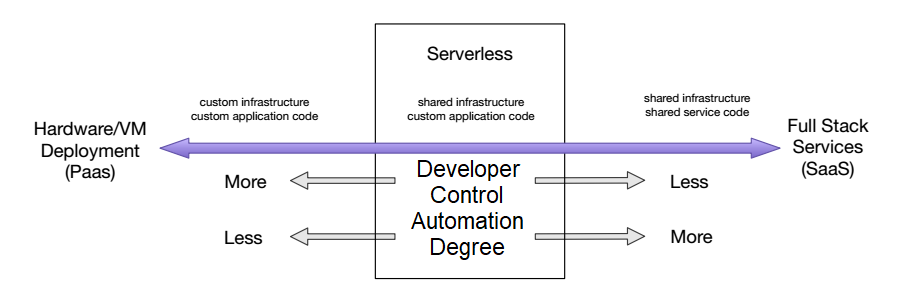
\includegraphics[width=0.9\textwidth]{figs/DeveloperControl.png}
	\caption{Automation degree in the XaaS taxonomy and the situation of serverless computing (adapted from~\cite{baldini2017serverless})}
	\label{fig:developer-control-serverless}
\end{figure}

On the opposite extreme are the PaaS and SaaS models, where the developer is unaware of any infrastructure and uses pre-packaged applications and services. Consequently, he no longer has control since the infrastructure provision is completely automated. In the middle, where serverless lives, the application developer has control over the code they deploy into the Cloud, though that code has to be written in the form of stateless functions.  The operational aspects of deployment and maintenance are completely automated, fault-tolerant and
auto-scaling. In particular, the code may be scaled to zero where no servers are actually running when the user's function code is not used, and there is no cost to the user. This is in contrast to PaaS solutions where the user is often charged even during idle periods~\cite{baldini2017serverless}.



%provide what is been called as \textit{Functions as a Service} (FaaS). A FaaS is a realization of the serverless paradigm in which stateless functions  


\subsection{Edge Computing and Low-Latency Applications}

Edge computing predicts the displacement of computing power to the network edge. Cloudlets~\cite{CLOUDLETS} have been first presented as mobile cloud servers which can be positioned at strategic locations with expected high density of (e.g., at concert halls, stations) or areas with temporary infrastructure limitations (e.g., after disasters). In contrast, mobile edge computing (MEC)~\cite{MEC} relies on cellular infrastructure to enable a low-latency communication between mobile devices and edge servers. 

In addition to the aforementioned types of edge computing, in this paper we explore the usage of \textit{local-edge} as servers deployed as part of a building infrastructure to further improve the computational power of nearby devices. Differently from classical \textit{on-premise} servers, local-edge should benefit from the automation and other characteristics of the A3-E model. As a result, local-edge servers can be seen as automated black boxes requiring no manual maintenance.
